
%% bare_conf.tex
%% V1.3
%% 2007/01/11
%% by Michael Shell
%% See:
%% http://www.michaelshell.org/
%% for current contact information.
%%
%% This is a skeleton file demonstrating the use of IEEEtran.cls
%% (requires IEEEtran.cls version 1.7 or later) with an IEEE conference paper.
%%
%% Support sites:
%% http://www.michaelshell.org/tex/ieeetran/
%% http://www.ctan.org/tex-archive/macros/latex/contrib/IEEEtran/
%% and
%% http://www.ieee.org/

%%*************************************************************************
%% Legal Notice:
%% This code is offered as-is without any warranty either expressed or
%% implied; without even the implied warranty of MERCHANTABILITY or
%% FITNESS FOR A PARTICULAR PURPOSE! 
%% User assumes all risk.
%% In no event shall IEEE or any contributor to this code be liable for
%% any damages or losses, including, but not limited to, incidental,
%% consequential, or any other damages, resulting from the use or misuse
%% of any information contained here.
%%
%% All comments are the opinions of their respective authors and are not
%% necessarily endorsed by the IEEE.
%%
%% This work is distributed under the LaTeX Project Public License (LPPL)
%% ( http://www.latex-project.org/ ) version 1.3, and may be freely used,
%% distributed and modified. A copy of the LPPL, version 1.3, is included
%% in the base LaTeX documentation of all distributions of LaTeX released
%% 2003/12/01 or later.
%% Retain all contribution notices and credits.
%% ** Modified files should be clearly indicated as such, including  **
%% ** renaming them and changing author support contact information. **
%%
%% File list of work: IEEEtran.cls, IEEEtran_HOWTO.pdf, bare_adv.tex,
%%                    bare_conf.tex, bare_jrnl.tex, bare_jrnl_compsoc.tex
%%*************************************************************************

% *** Authors should verify (and, if needed, correct) their LaTeX system  ***
% *** with the testflow diagnostic prior to trusting their LaTeX platform ***
% *** with production work. IEEE's font choices can trigger bugs that do  ***
% *** not appear when using other class files.                            ***
% The testflow support page is at:
% http://www.michaelshell.org/tex/testflow/



% Note that the a4paper option is mainly intended so that authors in
% countries using A4 can easily print to A4 and see how their papers will
% look in print - the typesetting of the document will not typically be
% affected with changes in paper size (but the bottom and side margins will).
% Use the testflow package mentioned above to verify correct handling of
% both paper sizes by the user's LaTeX system.
%
% Also note that the "draftcls" or "draftclsnofoot", not "draft", option
% should be used if it is desired that the figures are to be displayed in
% draft mode.
%
\documentclass[conference]{IEEEtran}

\usepackage{amsmath}
\usepackage{url}
\usepackage{cite}
\usepackage{graphicx}
\usepackage{color}
\usepackage{microtype}
\usepackage{units}
\usepackage{graphicx}
\usepackage{multirow}
\usepackage{paralist}
\usepackage[keeplastbox]{flushend}
\usepackage{tabularx}

% Add the compsoc option for Computer Society conferences.
%
% If IEEEtran.cls has not been installed into the LaTeX system files,
% manually specify the path to it like:
% \documentclass[conference]{../sty/IEEEtran}

\begin{document}
%
% paper title
% can use linebreaks \\ within to get better formatting as desired
\title{Learned Features for the Assessment of\\ Percussive Music Performances}

% author names and affiliations
% use a multiple column layout for up to three different
% affiliations
\author{\IEEEauthorblockN{Chih-Wei Wu}
\IEEEauthorblockA{Center for Music Technology\\
Georgia Institute of Technology\\
Atlanta, Georgia 30332\\
Email: cwu307@gatech.edu}
\and
\IEEEauthorblockN{Alexander Lerch}
\IEEEauthorblockA{Center for Music Technology\\
Georgia Institute of Technology\\
Atlanta, Georgia 30332\\
Email: alexander.lerch@gatech.edu}\\}

% use for special paper notices
%\IEEEspecialpapernotice{(Invited Paper)}




% make the title area
\maketitle


\begin{abstract}
The automatic assessment of (student) music performance involves the characterization of the audio recordings and the modeling of human judgments. To build a computational model that provides a reliable assessment, the system must take into account various aspects of a performance including technical correctness and aesthetic standards. While some progress has been made in recent years, the search for an effective feature representation remains open-ended. In this study, we explore the possibility of using learned features from sparse coding. Specifically, we investigate three sets of features, namely a baseline set, a set of designed features, and a feature set learned with sparse coding. In addition, we compare the impact of two different input representations on the effectiveness of the learned features. The evaluation is performed on a dataset of annotated recordings of students playing snare exercises. The results imply the general viability of feature learning in the context of automatic assessment of music performances.   
\end{abstract}
% IEEEtran.cls defaults to using nonbold math in the Abstract.
% This preserves the distinction between vectors and scalars. However,
% if the conference you are submitting to favors bold math in the abstract,
% then you can use LaTeX's standard command \boldmath at the very start
% of the abstract to achieve this. Many IEEE journals/conferences frown on
% math in the abstract anyway.

% no keywords

% For peer review papers, you can put extra information on the cover
% page as needed:
% \ifCLASSOPTIONpeerreview
% \begin{center} \bfseries EDICS Category: 3-BBND \end{center}
% \fi
%
% For peerreview papers, this IEEEtran command inserts a page break and
% creates the second title. It will be ignored for other modes.
\IEEEpeerreviewmaketitle



\section{Introduction}
Music performance is a sequence of actions that integrates both cognitive and motor skills. Starting from the musical ideas, this process of converting thoughts into movements is, as pointed out by Palmer \cite{Palmer1997}, among the most skill-intensive actions produced by human beings. To cultivate these skills, the qualitative assessment by peers and teachers is an essential pedagogical component in music education. A systematic assessment that is able to facilitate improvements usually requires careful examination of different aspects of a performance, such as technical correctness and alignment with aesthetic ideals. This task, however, is extremely difficult due to its subjective nature. As a result, human raters tend to exhibit a large variance in terms of their severity, rating scale, and the interpretation of rating categories \cite{Wesolowski2016}; the bias of the raters and the ill-defined categories, as suggested by Thompson and Williamon \cite{Thompson2003}, could adversely impact both the discriminability and the fairness of assessment. A computational approach that provides consistent and repeatable feedback, as illustrated in Fig.~\ref{fig:basic_idea}, might offer a potential solution to this issue and enhance the students' learning experience. 

\begin{figure}
\centering
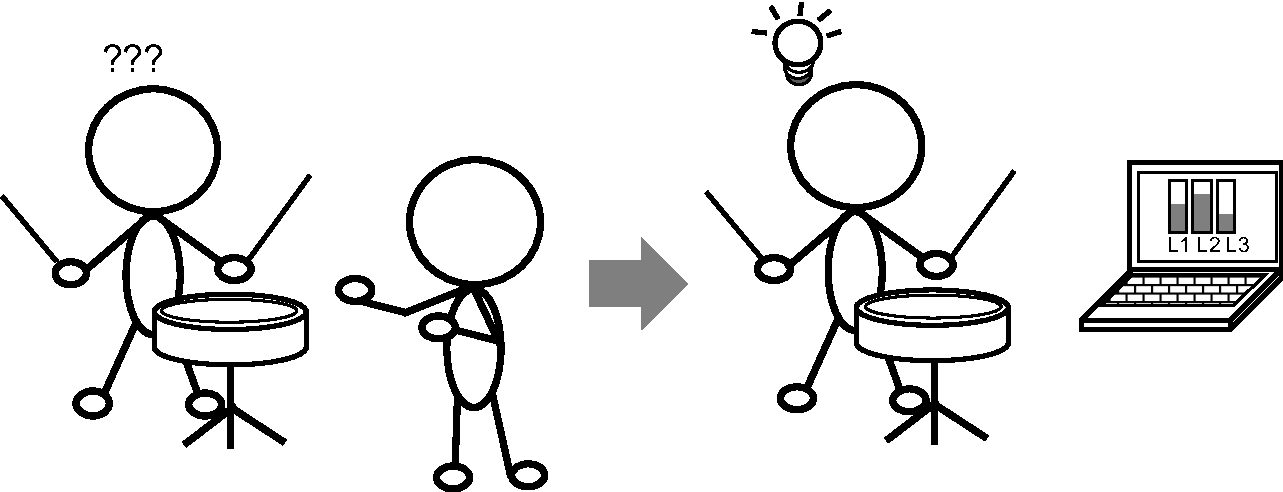
\includegraphics[width = 8 cm]{./figs/basic_idea.pdf}
\caption{The concept of automatic music performance assessment systems.}
\label{fig:basic_idea}
\end{figure}


With recent advances in the field of Music Information Retrieval (MIR) for tasks such as music transcription \cite{Benetos2013} and source separation \cite{Huang2014}, the realization of intelligent music systems with reliable functionality became plausible, opening up new possibilities for music education \cite{Dittmar2012}. Commercial software such as SmartMusic\footnote{http://www.smartmusic.com Last access: 2017/10/15} and Yousician\footnote{http://yousician.com Last access: 2017/10/15} both showcase how automatic assessment tools could enhance the music learning process with more flexible practice sessions and individualized feedback. These efforts, while providing rudimentary solutions to the users, still fall short in characterizing non-technical aspects of a performance. We hypothesize that this limitation originates from the design of the audio features. In MIR, a set of well-established features has proven to be surprisingly successful in applications such as music genre classification \cite{Tzanetakis2002}, music emotion recognition \cite{Kim2010}, and drum sound classification \cite{Herrera2003}, however, using the same features for other tasks such as music performance assessment has been shown lead to sub-optimal performance \cite{Wu2016, Vidwans2017}. %, and the fine-tuning of the features could be difficult and time-consuming.

In this paper, we explore the possibility of applying unsupervised feature learning in the context of music performance assessment. In particular, we compare the effectiveness of a set of baseline features, designed features, and learned features in assessing students' snare drum performances from a large set of recordings of the Florida all-state auditions. 
%{\textcolor{red} {maybe some comment here about how this can help understanding music, music performance, and music cognition, just to make it more 'semantic'}} 
{{A successful set of features would clearly describe the acoustic events rendered by the performers, providing a good foundation for studying the connection between music performance and its corresponding assessment given by the human judges.}}
Therefore, the goal of this paper is to find optimal features for characterizing percussive instrument performances.

The contributions of this paper include:
\begin{enumerate}[(i)]
	\item   new insights into the viability of applying feature learning to the problem of automatic music performance assessment, 
    \item   a new input representation that characterizes percussive instrument performances for feature learning purposes, and 
    \item   the demonstration of potential improvements in predicting judges' ratings using the proposed method.
    %\item   {\color{red}what about the whole domain knowledge argument?}
\end{enumerate} 

The remainder of this paper is structured as follows: Section~\ref{sec:relatedwork} presents the related work in automatic music performance assessment and feature learning. In Sect.~\ref{sec:method}, we introduce our proposed method. The experiment setup and results are described in Sect.~\ref{sec:experiments}. Finally, the conclusion and future directions are presented in Sect.~\ref{sec:conclusion}.

\section{Related Work}\label{sec:relatedwork}
% MPA with designed features
Music Performance Analysis (MPA) is a research field that concerns the study of the acoustic rendition of a musical score or idea \cite{lerch_software-based_2009}. 
%{\textcolor{red}{We have space, so why don't we fill it a bit with more info about music performance, such as how two performances of the same piece of music are not the same, what the parameters/dimensions are in which they are different etc.}} 
{{Instead of analyzing the intentions of the composer from the symbolic representation of a music composition, MPA focuses on interpreting the artistic decisions made by the performers during their music performance. For example, the same score can be played in different tempi or with different dynamics, resulting in performances with various levels of expressiveness. One of the main challenges of MPA, therefore, is to associate these expressions with human perception in a musically meaningful way.}}

To automate the process of MPA, a system must handle the extraction and interpretation of the important parameters of music performances. In the early research, most of the analysis was performed on symbolic data extracted from external sensors or MIDI devices. Recently, the focus has gradually shifted to the analysis of audio recordings. The basic approach to this problem usually involves the careful design of audio features that are capable of extracting the most relevant information in different contexts. For instance, Nakano presented an automatic system that evaluates the singing skill of the users \cite{Nakano2006a}; by characterizing the performances through pitch interval accuracy and vibrato features, the system was able to classify the performance into the two classes \textit{good} and \textit{poor}. 
%Barbancho et al.\  present a system that identifies violin techniques such as pizzicato and vibrato, using both time-domain and spectral features\cite{Barbancho2009}. With a hierarchical decision flow, the system differentiates seven playing techniques. {\textcolor{red} {hmm. why is the barbancho reference relevant?}}
Abe{\ss}er et al.\ propose a system that automatically assesses the quality of vocal and instrumental performances of 9th and 10th graders \cite{Abeßer2013}. Features representing the pitch, intonation, and rhythmic correctness are designed to quantify the students' performances. They report that the system is able to predict four different performance qualities with occasional confusions between the adjacent classes. 
In a system that identifies the common mistakes by the flute beginners, Han and Lee propose to use features such as MFCCs with sparse filtering for detecting events such as poor blowing and misfingering\cite{Han2014}. %{\color{red}what kind of features?} 
More recently, Wu et al.\  and Vidwans et al.\ propose to assess students' instrumental performances using a set of features derived from pitch, amplitude, and inter-onset interval histograms\cite{Wu2016, Vidwans2017}. The evaluation results show reasonable correlation between the model predictions and expert judges' ratings. 

All of the above mentioned systems use custom-designed features in the analysis pipeline. This approach, while translating existing music domain knowledge into machine operations, might also strip away important information that resides in the data. Feature learning, on the other hand, allows an algorithm to find the most fitting features based on given input representations. Several feature learning methods have been found successful in music related applications, especially for the task of music genre recognition. For example, Lee et al.\  applied convolutional Deep Belief Networks (DBNs) to magnitude spectrograms to learn features \cite{Lee2009a}; the evaluation results show that the learned features outperform conventional audio features in recognizing music genre. 
Similarly, Hamel and Eck demonstrate that a DBN is able to derive features that achieve state-of-the-art performance in music genre recognition \cite{Hamel2010}. 
Henaff et al.\  apply Sparse Coding (SC) to the log spectrogram and use the learned features to train a SVM classifier. The evaluation results also indicate the effectiveness of the learned features for recognizing music genres \cite{Henaff2011}. 
Nam et al.\  further introduce a pre-processing pipeline that improves the SC feature learning \cite{Nam2012}; the evaluation results on a music tagging dataset compare favorably against the commonly used audio features. More recently, SC-derived features have also been shown effective for music genre recognition \cite{Hsu2016} and music emotion recognition \cite{OBrien2015}. 

Based on the findings in the previous work, both DBNs and SC seem to be useful approaches for feature learning in music related tasks. Compared with DBNs, however, SC seems to have a broader range of applications in addition to the MGR task. Therefore, in this study, we propose to explore the viability of applying sparse coding for music performance assessment.
%{\color{red}what's with all the pipelines in this paper?}
%{\color{red}this is a bit too fuzzy to me. what do you mean exactly? I would probably just write that you might strip away important information...}

\section{Method}\label{sec:method}
\subsection{System Overview}
The proposed system comprises both a training and a testing phase. As shown in Fig.~\ref{fig:flowchart}, the training phase starts by transforming each audio recording into the input representation; the input representations are collected for the training data and passed to the feature learning block. In the feature learning step, the feature extractor is derived by solving an optimization problem across the entire dataset, and the corresponding feature vector for each recording is calculated. Finally, the features are used to train a regression model that minimizes the loss between the model prediction and the ground truth (judges' ratings) for each recording, along with an outlier removal step to refine the model. 

\begin{figure}
\centering
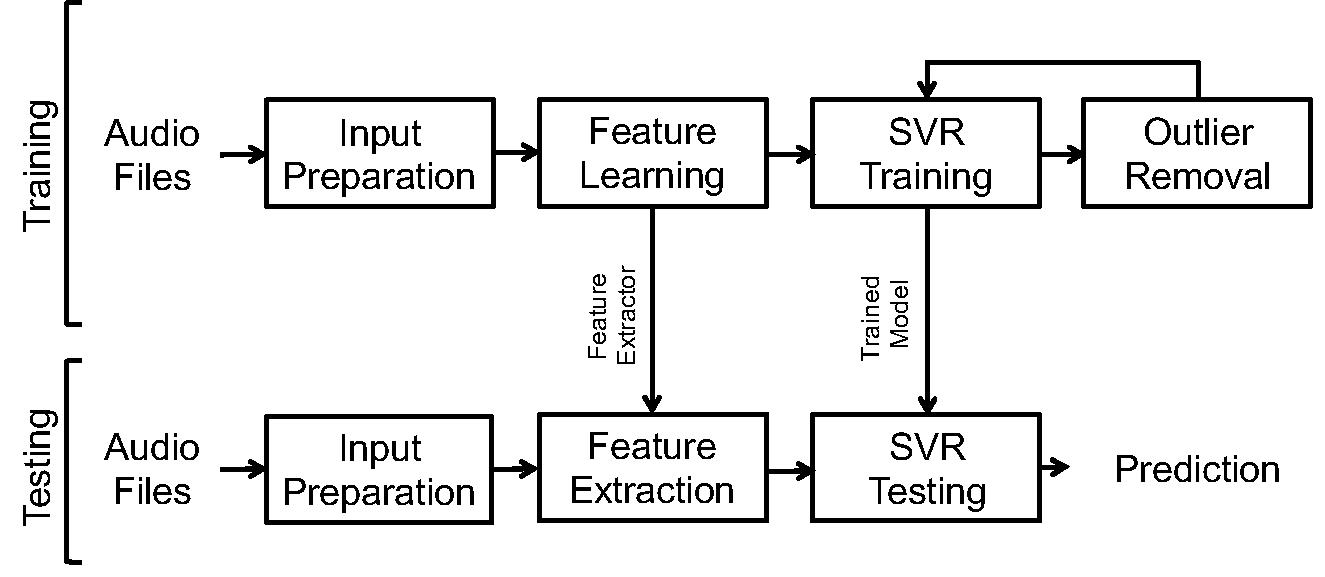
\includegraphics[width = 8 cm]{./figs/flowchart.pdf}
\caption{The flowchart of the proposed method.}
\label{fig:flowchart}
\end{figure}

In the testing phase, a similar procedure is followed for each recording to prepare the input representation and extract features using the derived feature extractor. The resulting feature vector is then used to predict the judges' ratings with the pre-trained regression model. In the following sections, more details of each processing step are presented. 

\subsection{Input Preparation}\label{subsec:input}
% talk about two different inpu representations I tried
% STFT & IOI hist
The goal of the input preparation step is to normalize, reduce the amount of data, and to convert the data into meaningful input representations. First, audio recordings are down-mixed to mono and resampled to a sampling rate of \unit[22.05]{kHz} after decoding. All files are normalized to a numerical range between -1 and 1. Finally, two different matrix representations are computed, namely the Short-Time Fourier Transform (STFT) and a Local Histogram Matrix (LHM). 

\subsubsection{STFT}\label{subsec:stft}
The STFT is computed using a block size of 512 samples with 75\% overlapping blocks; a Hann window is applied to each block. Only the magnitude spectrogram is used and the phase information is discarded. The resulting spectrogram $M_\mathrm{stft}$ is a $m \times n$ matrix, in which $m = 257$ and $n$ equals the number of blocks. This input representation has been referred in some related literatures as a baseline \cite{Su2014Guitar, Su2014Violin}. % {\textcolor{red} {This confuses me a bit. This is the baseline comparison for the SC literature? With what has it been compared?}} 

\subsubsection{LHM}
This input representation aims to capture the most important overall characteristics of the percussive instrument performances. The extraction process of the local histogram matrix is shown in Fig.~\ref{fig:hist_mat}. In order to extract the histogram, the input time-domain audio signal is first partitioned into non-overlapping local segments of length \unit[10]{s}. This length enables us to capture higher level structure such as music phrases. Within each segment, the Inter-Onset-Interval (IOI) histogram vector $\mathbf{v}_\mathrm{ioi}$, the amplitude histogram vector $\mathbf{v}_\mathrm{amp}$, and the averaged MFCC vector $\mathbf{v}_\mathrm{mfcc}$ is extracted.
Concatenating these vectors will result in local histogram matrix $M_\mathrm{lhm}$ that represents each individual recording. The definitions of these vectors are:
%{\color{red}now that I read it it sorta reminds of Thanos' paper (maybe not the one you co-authored)?}
\begin{figure}
    \centering
    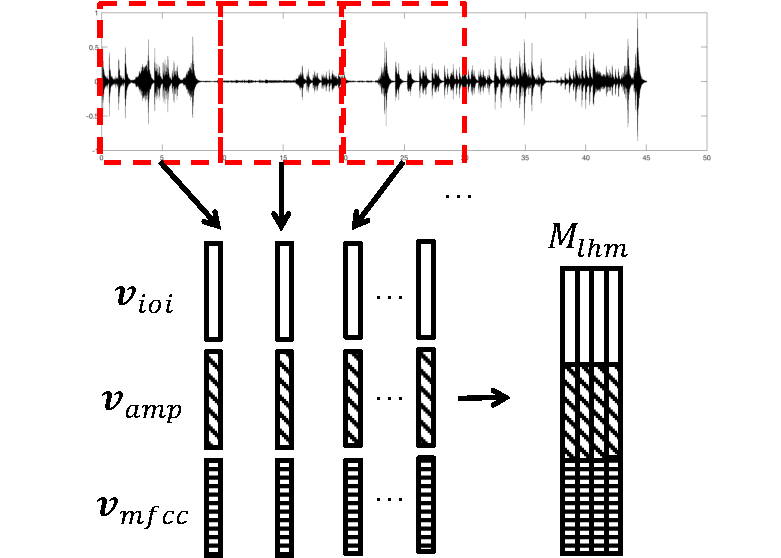
\includegraphics[width = 8 cm]{./figs/hist_mat.pdf}
    \caption{Illustration of the construction process of local histogram matrix; $\mathbf{v}_\mathrm{ioi}$ is the IOI histogram vector, $\mathbf{v}_\mathrm{amp}$ is the amplitude histogram vector, $\mathbf{v}_\mathrm{mfcc}$ is the averaged MFCCs vector, and $M_{lhm}$ is the local histogram matrix.}
    \label{fig:hist_mat}
\end{figure}

\begin{figure}
    \centering
    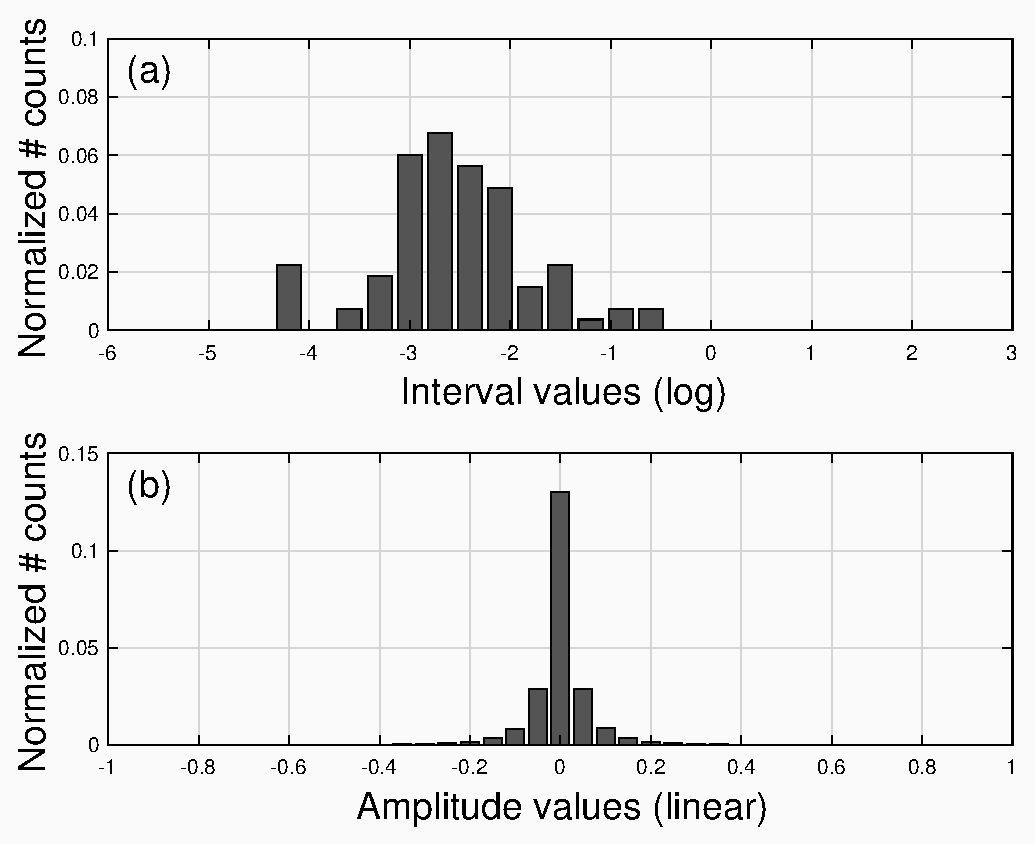
\includegraphics[width = 8 cm]{./figs/ioi_hist_examples.eps}
    \caption{An example of (a) an IOI histogram vector $\mathbf{v}_\mathrm{ioi}$ and (b) an amplitude histogram vector $\mathbf{v}_\mathrm{amp}$. All histograms are normalized by the total number of counts and can be interpreted as probability distributions.} 
    \label{fig:ioi_hist_example}
\end{figure}




\begin{enumerate}[(i)]
    \item   \textbf{IOI histogram vector ($\mathbf{v}_\mathrm{ioi}$)}: the onset times, i.e., the start times of individual drum events are estimated within the local segment using a standard spectral flux novelty function and an adaptive median threshold for peak picking; the implementation follows the description in \cite{Lerch2012} and results in a vector $onset(i)$ in which $i$ is the onset index. The IOI sequence is calculated by $IOI = diff(onset(i))$, followed by a non-linear transformation $IOI_\mathrm{ln} = ln(IOI)$. Since the ratios between onset intervals are frequently powers of 2 (e.g., an 8th note is twice as long as a 16th note), this transformation helps to characterize the rhythmic patterns within a musically more meaningful numerical range. Next, the $\mathbf{v}_\mathrm{ioi}$ is computed by estimating the histogram from the $IOI_\mathrm{ln}$ with a pre-defined range and resolution, determined through data observation in pilot experiments. Finally, the $\mathbf{v}_\mathrm{ioi}$ is normalized by dividing the total number of onsets in the entire recording. The resulting $\mathbf{v}_\mathrm{ioi}$ is a column vector with dimensionality $d_\mathrm{ioi} = 31$. An example of  $\mathbf{v}_\mathrm{ioi}$ is shown in Fig.~\ref{fig:ioi_hist_example}(a).

    \item   \textbf{Amplitude histogram vector ($\mathbf{v}_\mathrm{amp}$)}: following a procedure similar to the one described above, $\mathbf{v}_\mathrm{amp}$ is calculated by estimating the histogram of the amplitude values within the local segment. The range of the histogram is from -1 to 1 with a resolution of 0.05 between the consecutive bins. The $\mathbf{v}_\mathrm{amp}$ is normalized by the total number of samples in the entire recording. This is represented as a column vector of dimensionality $d_\mathrm{amp} = 41$. An example of  $\mathbf{v}_\mathrm{amp}$ is shown in Fig.~\ref{fig:ioi_hist_example}(b).

    \item   \textbf{Averaged MFCC vector ($\mathbf{v}_\mathrm{mfcc}$)}: given a local segment, the first 13 Mel Frequency Cepstral Coefficients (MFCCs) are computed using the same block size and overlap as defined in Sect.~\ref{subsec:stft}, which leads to a $13 \times n_\mathrm{b}$ matrix where $n_\mathrm{b}$ is the number of blocks within the segment. Next, the $\mathbf{v}_\mathrm{mfcc}$ is calculated by averaging the MFCC matrix across the $n_\mathrm{b}$ blocks, resulting in a column vector of dimensionality $d_\mathrm{mfcc} = 13$. 
\end{enumerate} 

The same procedure will repeat for each 10-second local segment, resulting in the final matrix $M_\mathrm{lhm}$ is a $m' \times n_\mathrm{s}$ matrix,  in which 
\begin{equation}
    m' = d_\mathrm{ioi} + d_\mathrm{amp} + d_\mathrm{mfcc} = 85
\end{equation}%
and $n_\mathrm{s}$ is the number of local segments.


\subsection{Feature Learning}\label{subsec:feat_learn}
% sparse coding
The feature learning algorithm used in this paper is Sparse Coding (SC), which can be expressed as %Eq.~\ref{eq:lasso}
\begin{equation}\label{eq:lasso}
\hat{\alpha} = \mathop{\mathrm{argmin}}_\alpha \frac{1}{2} \| X - D\alpha \|_{2}^{2} + \lambda \| \alpha \|_{1}, 
\end{equation}
%
with $X \in R^{ m \times n}$ as the input matrix, i.e., $M_\mathrm{stft}$ or $M_\mathrm{lhm}$. $D$ is the $m \times k$ dictionary matrix, $\alpha$ is the $k \times n$ sparse matrix, $\lambda$ is the sparsity coefficient, $n$ is the number of local segments, and $k$ is the user-defined dictionary size. 

This $\ell_1$ regularized Least Absolute Shrinkage and Selection Operator (LASSO) problem can be solved by the Least Angle Regression (LARS) algorithm efficiently\cite{Efron2004}, in which the dictionary $D$ and the sparse matrix $\alpha$ can be learned by iteratively minimizing the reconstruction loss. Finally, the resulting dictionary $D$ can be considered as the feature extractor, where the corresponding sparse representation $\alpha$ can be used to compute the features. 

To compute the final feature vector that represents each audio recording, our system first learns an universal dictionary $D_\mathrm{all}$ from the entire dataset. This can be done by concatenating the $M_\mathrm{stft}$ or $M_\mathrm{lhm}$ across all the training files, and solve the LASSO optimization problem on the concatenated matrix $X_\mathrm{all}$. %{\textcolor{red}{should we maybe just rename X to M?}} 
Next, the $\alpha_\mathrm{individual}$ is estimated from each recording by substituting the $X$ in Eq.~\ref{eq:lasso} with the input representation of an individual file $X_\mathrm{individual}$ while keeping the $D = D_\mathrm{all}$ fixed throughout the optimization process. The resulting $\alpha_{individual}$ is a $k \times n$ sparse matrix. Finally, $\alpha_\mathrm{individual}$ is aggregated using mean and standard deviation across $n$ segments, producing a feature vector $\mathbf{\alpha_\mathrm{final}} = [mean(\alpha_\mathrm{individual}); std(\alpha_\mathrm{individual})]$ with a dimensionality of $d_\mathrm{final} = 2 \times k$. $[ ; ]$ is a vector concatenation operator.

In our experiment, the Matlab implementation for SC from the open source library SPAMS\footnote{http://spams-devel.gforge.inria.fr Last accessed: 2017/10/15}\cite{Mairal2009a} is used. For parametrization, $k = \{32, 64, 128\}$ has been tested, and the sparsity coefficient $\lambda = \nicefrac{1}{\sqrt{block\, size}}$ is applied. 

\subsection{Regression Model}
% SVR training and outlier removal
The regression model used is Support Vector Regression (SVR) with a linear kernel. The Matlab implementation of this algorithm from the  open source library  libsvm \cite{Chang2011}, is used with default settings. Due to the limited size of sample pool (see Sect.~\ref{subsec:dataset} for more details), a Leave One Out (LOO) cross-validation scheme is applied to our evaluation process. The main idea of LOO is to sequentially select one sample from the pool as test data and use the rest of the pool as training data until all the samples have been tested. Additionally, an outlier removal process is implemented by iteratively removing the sample with the largest residual between the prediction and the actual label until 5\% of the entire data is eliminated. This process potentially helps the regressor to better capture the underlying patterns of the data.  

\section{Experiments}\label{sec:experiments}
\subsection{Dataset}\label{subsec:dataset}

%% ===== OVERVIEW OF FBA DATASET
%\begin{table}
%\centering
%\caption{An overview of numbers of student recordings in FBA dataset from 2013 to 2015}
%\begin{tabularx}{\columnwidth}{c@{\extracolsep{\fill}}cccc}
%%\begin{tabular}{ccccc}
%\hline
%\multirow{2}{*}{\textbf{Year}}       & \multicolumn{3}{c@{\extracolsep{\fill}}}{\textbf{Group}}                                                                                                                                                                                       & \multirow{2}{*}{\textbf{Total}}      \\ \cline{2-4}
%                                     & \textbf{\begin{tabular}[c]{@{}c@{}}Middle\\ School\end{tabular}}       & \textbf{\begin{tabular}[c]{@{}c@{}}Concert\\ Band\end{tabular}}       & \textbf{\begin{tabular}[c]{@{}c@{}}Symphonic\\ Band\end{tabular}}       &                                      \\ \hline
%2013                                 & 1099                                                                   & 984                                                                   & 1200                                                                    & 3283                                 \\
%2014                                 & 1133                                                                   & 1052                                                                  & 1368                                                                    & 3553                                 \\
%2015                                 & 1106                                                                   & 1102                                                                  & 1378                                                                    & 3586                                 \\ \hline
%\multicolumn{5}{c}{\textbf{List of all instruments}}                                                                                                                                                                                                                                                   \\ \hline
%\multicolumn{5}{c}{\begin{tabular}[c]{@{}c@{}}Alto Sax, Baritone Sax, Bass Clarinet, \\ Bass Trombone, Bassoon, Bb Clarinet, \\ Bb Contrabass Clarinet, Eb Clarinet, English Horn, \\ Euphonium, Flute, French Horn, Oboe, \\ Percussion, Piccolo, Tenor Sax,\\  Trombone, Trumpet, Tuba\end{tabular}} \\ \hline
%\end{tabularx}
%\label{tab:fba_all}
%\end{table}
%{\color{red}my suggestion is to make all tables column width, it just looks nicer}


% information about the overall dataset
The dataset used for this study is provided by the Florida Bandmasters Association (FBA). This dataset contains audio recordings from the Florida all-state auditions of three groups of students: middle school (7th and 8th graders), concert band (9th and 10th graders), and symphonic band (11th and 12th graders) for three consecutive years (2013 to 2015). A total number of 19 types of instruments are included in the auditions. As a result, this dataset can be split into different subsets of recordings by their year, group, and instrument (e.g., 2013, middle school, clarinet). Each subset contains up to 180 recordings of student performances.  

In each recording, a student is required to perform several exercises, such as technical etude, lyrical etude, chromatic scale, 12 major scales, and sight-reading. Each exercise is graded by expert judges using assessment categories such as \textit{musicality}, \textit{note accuracy}, \textit{rhythmic accuracy}, \textit{tone quality}, \textit{artistry}, and \textit{articulation}. The number of judges and the grading criteria are not available. The maximum score of these categories vary from 5 to 40. In our experiments, all of the ratings are normalized to a range between 0 and 1 by dividing the score with the maximum allowed value of the corresponding category. %An overview of the FBA dataset is shown in Table \ref{tab:fba_all}. 
More information on the dataset can be found in our Github repository.\footnote{https://github.com/GTCMT/FBA2013, Last access: 2017/10/15}%\footnote{http://dummy.link}  

In this study, the focus is on assessing percussion performance. For percussion instruments, the audition session includes 5 different exercises, which are mallet etude, snare etude, chromatic scale (xylophone), 12 major scales (xylophone), and sight-reading (snare). To further narrow down the scope of this study, we use only the subset of middle school snare etude from all three years. This particular combination is selected for containing a comparably high number of students. As shown in Table \ref{tab:fba_snare}, a total number of 274 recordings of snare etude with an averaged duration of \unit[51.3]{s} is available for analysis. For this particular exercise, the assessment categories are musicality (L1) and rhythmic accuracy (L2).


%===== details of snare etude recordings
\begin{table}
\centering
\caption{Statics of the middle school snare etude from 2013 to 2015}
\begin{tabularx}{0.48 \textwidth}{c@{\extracolsep{\fill}}ccc}
%\begin{tabular}{cccc}
\hline
\multicolumn{4}{c}{\textbf{Middle school/ Percussion/ Snare Etude}}                                                                                                               \\ \hline
\textbf{Year} & \textbf{\#Students} & \textbf{\begin{tabular}[c]{@{}c@{}}Total Dur \\ (sec)\end{tabular}} & \textbf{\begin{tabular}[c]{@{}c@{}}Average Dur\\ (sec)\end{tabular}} \\ \hline
2013          & 98                  & 4953                                                                & 50                                                                    \\
2014          & 90                  & 4595                                                                & 51                                                                    \\
2015          & 86                  & 4608                                                                & 53                                                                    \\ \hline
\end{tabularx}
\label{tab:fba_snare}
\end{table}

\subsection{Experiment Setup}
This paper presents two experiments that highlight different characteristics of the proposed feature learning method in the context of assessing student snare drum performances. The goal of Experiment 1 is to compare the effectiveness of two different input representations (see Sect.~\ref{subsec:input}) for SC. For Experiment 2, the goal is to find the best combination of feature sets in order to achieve the highest performance. 

%{\color{red}would it be better if we stated the goal of these experiments right here?}

% Experiment 1: feature learning from two different input representations
In Experiment 1, the tested configurations are:% listed as follows: %{\color{red} are you sure you want to use the ``+'' for this? Because here it is more a specifier while below it's the combination of different feature sets}
\begin{enumerate}[(i)]
\item \textbf{SC (STFT)}: sparse coding features using STFT as input representations and
\item \textbf{SC (LHM)}: sparse coding features using LHM as input representations.
\end{enumerate}
Both configurations are tested using $k = \{32, 64, 128\}$.\\

% Experiment 2: comparison between different combination of feature sets
In Experiment 2, the regression model trained on the SC learned features using the proposed LHM with $k = 32$ is compared to two different sets of features, referred to as \textit{Baseline} and \textit{Designed} features, as proposed by Wu et al.~\cite{Wu2016}. The regression performance of the following feature set combinations is tested:
\begin{enumerate}[(i)]
\item \textbf{Baseline}: the standard spectral and temporal features such as spectral centroid, spectral rolloff, spectral flux, zero-crossing rate, and 13 MFCCs. The dimensionality is $d_\mathrm{baseline} = 68$.
\item \textbf{Designed}: the designed rhythmic and dynamic features derived from the IOI and amplitude histograms. These features involve the calculation of various statistics, such as crest, skewness, flatness, kurtosis, etc., directly from the histograms of the entire recording (compare \cite{Wu2016} for more details). The dimensionality is $d_\mathrm{designed} = 18$. 
%{\color{red} we could add more description here. Maybe it's a bit annoying to look this all up?}

\item \textbf{SC (LHM)}: see Sect.~\ref{subsec:feat_learn}. %{\color{red}why is this ``proposed'' and not lhm?}
\item \textbf{Designed + Baseline}: a combined feature set consisting of both baseline and designed features. %{\color{red}I changed the naming order --- I just like it better that way. Could you adapt the plot?} 
\item \textbf{SC + Baseline}:  a combined feature set consisting of both SC and baseline features.
\item \textbf{SC + Designed}:  a combined feature set consisting of both SC and designed features.
%\item \textbf{All}: a combination of all three sets of features
\end{enumerate}

\subsection{Metrics}
The performance of the models is investigated using the following standard statistical metrics: the Pearson correlation coefficient $r$ and the coefficient of determination, i.e., $R^{2}$. These metrics are commonly used to evaluate the strength of the relationship between the regression predictions and ground truth. Details of the mathematical formulations can be found in \cite{McClave2003}. 

\subsection{Experiment Results}
\begin{table}
\centering
\caption{Evaluation results for Experiment 1: L1 represents musicality, and L2 represents rhythmic accuracy. The higher is better.}
\begin{tabularx}{\columnwidth}{c@{\extracolsep{\fill}}ccccc}
%\begin{tabular}{cccccc}
\hline
\multicolumn{2}{c}{Input Representation}                                             & \multicolumn{2}{c}{STFT} & \multicolumn{2}{c}{LHM}       \\ \hline
\begin{tabular}[c]{@{}c@{}}Dictionary \\ Size\end{tabular} & Metrics                 & L1         & L2          & L1            & L2            \\ \hline
\multirow{2}{*}{k = 32}                                    & r                       & 0.34       & 0.19        & \textbf{0.65}          & \textbf{0.57} \\
                                                           & $R^{2}$ & 0.08       & -0.02       & \textbf{0.41}          & \textbf{0.29} \\ \hline
\multirow{2}{*}{k = 64}                                    & r                       & 0.41       & 0.26        & \textbf{0.70} & \textbf{0.50}          \\
                                                           & $R^{2}$ & 0.11       & -0.00       & \textbf{0.45} & \textbf{0.06}          \\ \hline
\multirow{2}{*}{k = 128}                                   & r                       & \textbf{0.41}       & 0.28        & 0.33          & \textbf{0.34}          \\
                                                           & $R^{2}$ & \textbf{0.08}       & \textbf{-0.07}       & -0.08         & -0.78         \\ \hline
\end{tabularx}
\label{tab:exp1}
\end{table}

% LHM outperform STFT overall. STFT can't capture the temporal information 
% when k is large, both perform poorly (274 samples, when k = 128, the feature has a d = 2*k = 256) which could bring a lot of noise
% when k = 32, the improvement is the largest. 
In this section, the evaluation results of both experiments are presented and discussed. Since all of the correlation results are significant ($p\ll 0.05$), their p-values are not reported.  

%{\color{red}why is there nothing bold in the last two rows?})
%{\color{red}you mean if you approximate the STFT unshuffled?}
%{\color{red}just a quick question then: why not change feature aggregation to reflect this? (just playing the reviewer here}
%{\color{red}wait: when did you talk about feature dimensionality before?}
The evaluation results of Experiment 1 are shown in Table~\ref{tab:exp1}. The following trends can be observed: first, the LHM input representation outperforms the STFT representation in almost every case. This result clearly shows that for this task, LHM is a more effective input representation than STFT. A likely explanation is that this discrepancy originates from the representations' capabilities of capturing temporal information. Since the STFT only represents the spectral content at various single instances, it does not encapsulate any temporal dependencies between meaningful audio events such as consecutive drums hits. This temporal information, while being likely to reside in the sparse matrix $\alpha$, will be lost after the feature aggregation. The absence of temporal information apparently poses a problem for SC to learn higher level music concepts such as rhythm. LHM, on the other hand, captures some temporal dependencies between the audio events with the IOI histograms. This allows for the rhythmic information to be translated into the SC dictionary and to reflect on the final features, leading towards a better performance. 
Second, both STFT and LHM perform poorly for the largest dictionary size with $k = 128$. The reason behind this degradation for both representations might be due to the limited size of the sample pool. When $k = 128$, the resulting feature dimensionality, as described in Sect.~\ref{subsec:feat_learn}, would be $k \times 2 = 256$. This will result in a feature matrix of $274 \times 256$ $(\text{students} \times \text{features})$, and the model could suffer from the curse of dimensionality \cite{Bishop2006}. One potential solution to this problem would be to apply dimensionality reduction methods such as Principle Component Analysis (PCA) or feature selection, however, this is out of the scope of this study. 
Third, when $k = 32$, the LHM has the largest improvement over STFT in both L1 and L2. This result might indicate a relationship between the best performing $k$ and the number of samples in the dataset.

% Experiment 2

\begin{figure*}
\centering
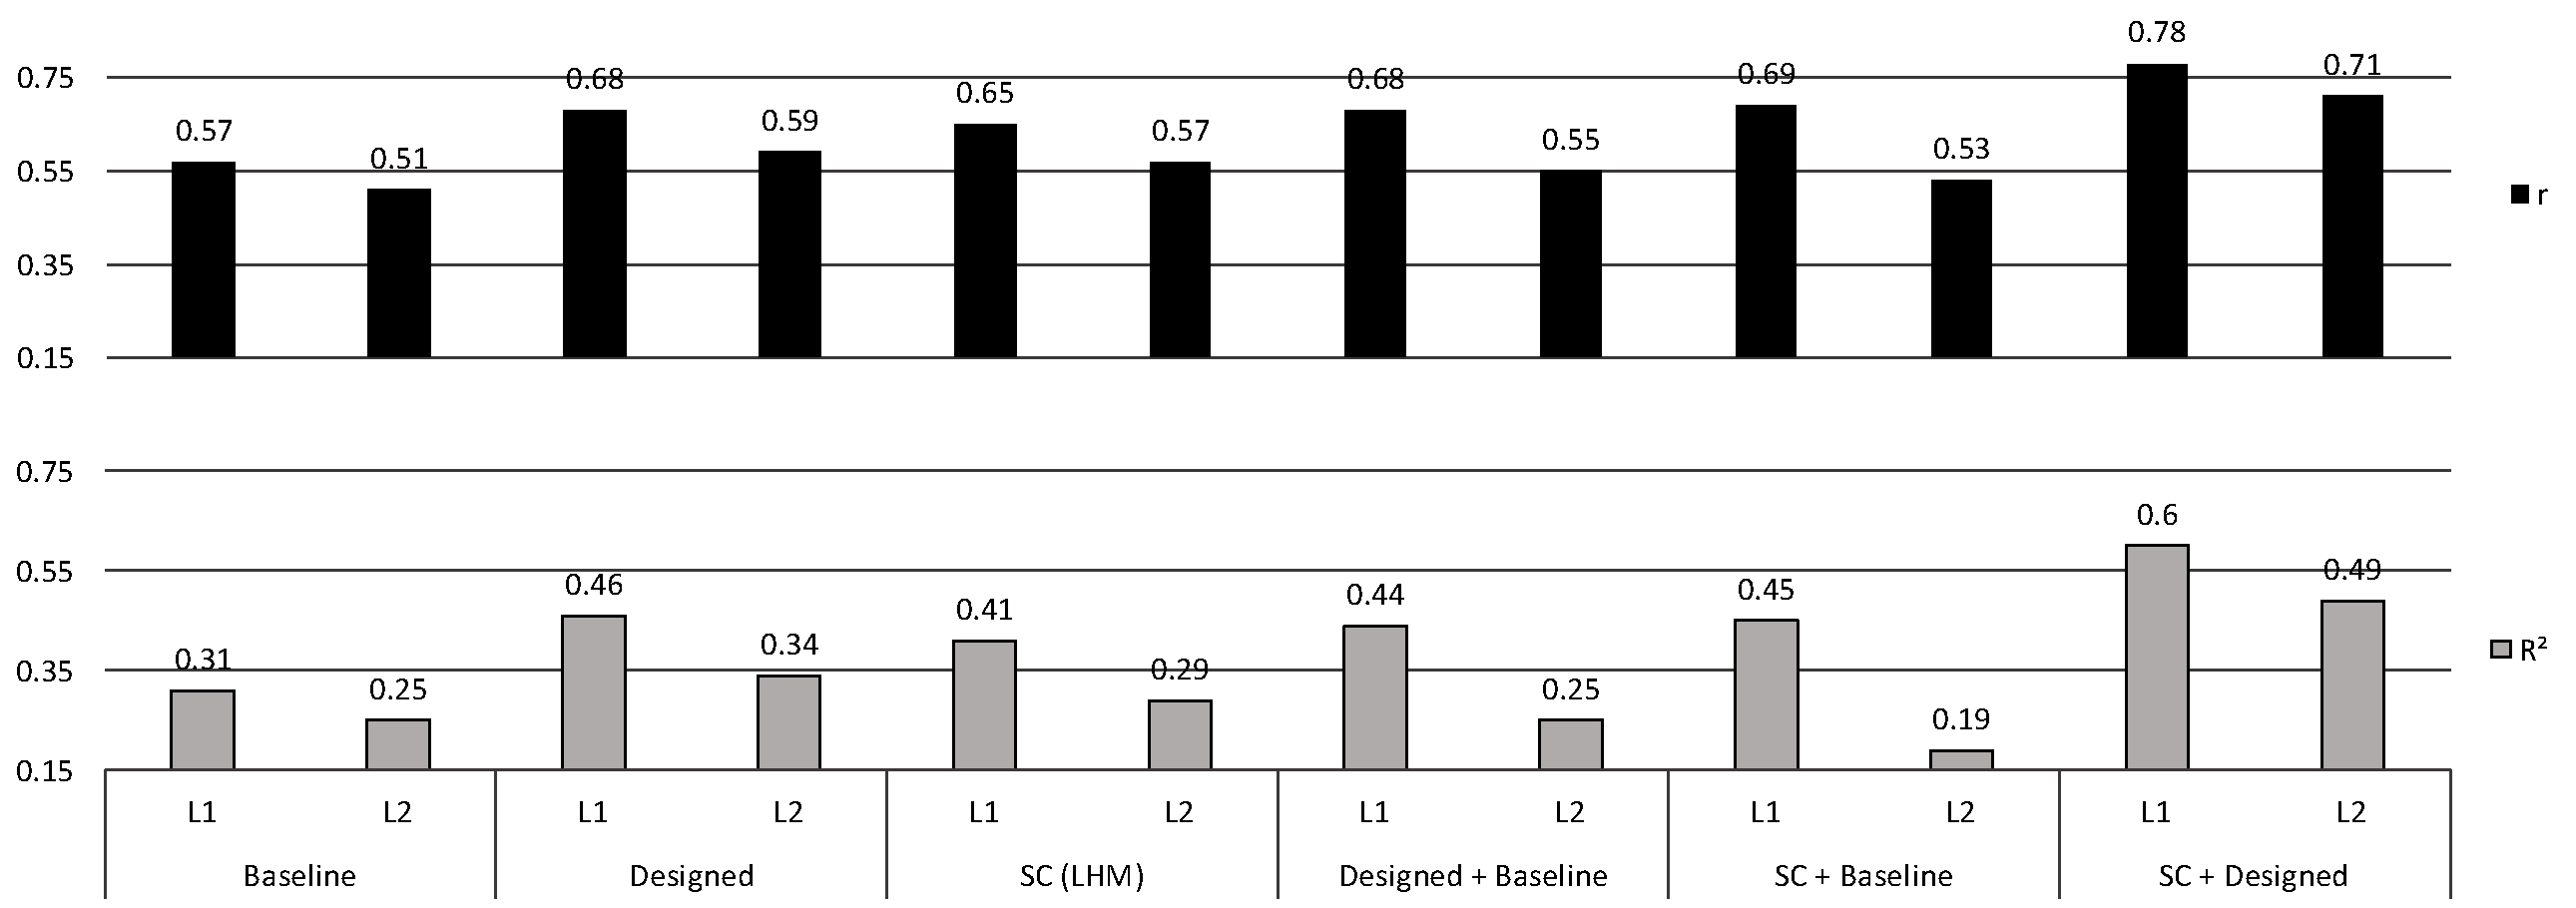
\includegraphics[width = 17.2 cm]{./figs/exp2_remake.pdf}
\caption{Evaluation results for Experiment 2 (top) $r$ (bottom) $R^{2}$}
\label{fig:exp2}
\end{figure*}



% Short summary

% first thing to 
The evaluation results of Experiment 2 are shown in Fig.~\ref{fig:exp2}. The first observation we can make is that both the designed and the SC features outperform the baseline features. This is in line with our expectations, as the baseline features are low-level instantaneous features that are not optimized to the task. %It is interesting to note, though, that the baseline features in this experiment still outperform the STFT SC features in Experiment 1. {\color{red}is there a reason for this? aggregation again? Or should we remove this comment?}
Second, the proposed SC features achieve comparable performance to the designed features. The fact that SC features perform similarly to the designed features is encouraging, suggesting the possibility of deriving viable features through feature learning with minimum effort in feature crafting. 
Third, when combined with baseline features, both designed and SC features exhibit almost no improvements. There exist two possible explanations for this. On the one hand, it could be that these features do not add any information that is not already in the other features. On the other hand, this issue could be similar to the situation in Experiment~1 when having a large $k$, as adding baseline features might induce the curse of dimensionality by introducing too many features to the current size of sample pool. %{\color{red}is facilitate the right word?}
Four, among all the tests in Experiment 2, the highest performance is achieved with the combination of designed and SC features. The result implies the effectiveness of SC features in capturing information that is non-redundant to the information provided by the designed features.
This demonstrates the potential of using feature learning methods to complement designed features due to the learned features' ability to capture relevant information not or incompletely modeled by features designed with expert knowledge.

A general observation that can be made from all experiment results is the superior model performance for L1 over L2. As discussed in \cite{Wu2016}, musicality is an abstract but holistic measure of the performance, and it is therefore more likely to reflect the overall perception of the judges and is more consistent across the years. %{\color{red}I think this could be extended if you wanted to. Both here and in the data section, possibly referring to the correlations between labels as well. Did you intentionally omit this? Also, I am really not sure if we can just say it's more consistently graded...}

% conclude from both experiments: musicality is easier to model
\section{Conclusion}\label{sec:conclusion}
% we show the importance of input representation prior to feature learning. The experiment results show that a good intermediate feature representation is important
This paper presents an unsupervised feature learning approach to derive features for assessing percussive instrument performances. Specifically, we propose to use a histogram-based input representation to SC in order to allow the sparse coding to take advantage of temporal rhythmic information. We could show that~---~for the task of performance assessment~---~this input representation outperforms an STFT-based input representation that is frequently used for feature learning approaches. The learned features perform comparable to expert-designed features for this task, and are able to capture task-relevant information that is not represented in the designed features, indicating the suitability of combining "traditional'' feature design methods with feature learning approaches for optimal performance.

In summary, the contributions of this work are: 
First, it provides insights into the selection of input representations for feature learning in the context of snare drum performance assessment, favoring representations inspired by domain knowledge over standard representations such as STFT. 
Second, the proposed learned features achieve comparable results with the designed features, demonstrating the viability of deriving competitive features with minimum effort in feature design. 
Finally, combining the designed features with the SC features, the highest performance can be achieved. This result suggests that learned features might be able to provide complementary information to the features designed with domain knowledge, further optimizing the performance of a given task. 

Possible future directions of this work include: 
\begin{enumerate}[(i)]
    \item   Evaluate and compare the efficiency of different feature learning algorithms. Methods such as DBN\cite{Hamel2010} and denoising autoencoders \cite{Vincent2008} may provide new insights into the finding of the best feature learning strategy for automatic performance assessment.
    \item   Adapt the proposed method to other types of instruments such as Brass or Woodwind instruments. The evaluation results on melodic instruments could lead to the refinement of the proposed feature learning scheme. 
    \item   Try to allocate more data. To further investigate the robustness and generality of this approach, more data is needed. Additionally, the increase in sample pool can also help the investigation into issues such as the relationship between dictionary size $k$ and the number of samples. This might lead to a better strategy for selecting the best performing dictionary size. 
\end{enumerate}

Music Performance Analysis and assessment is a multifaceted topic, and the traditional custom-designed features might not capture all information that is needed for a detailed analysis. Complementing the set of features with learned features is a promising direction that we intend to explore further.

% conference papers do not normally have an appendix


% use section* for acknowledgement
\section*{Acknowledgment}

The authors would like to thank the Florida Bandmasters Association for providing the dataset used in this study.

% trigger a \newpage just before the given reference
% number - used to balance the columns on the last page
% adjust value as needed - may need to be readjusted if
% the document is modified later
%\IEEEtriggeratref{8}
% The "triggered" command can be changed if desired:
%\IEEEtriggercmd{\enlargethispage{-5in}}

% references section

% can use a bibliography generated by BibTeX as a .bbl file
% BibTeX documentation can be easily obtained at:
% http://www.ctan.org/tex-archive/biblio/bibtex/contrib/doc/
% The IEEEtran BibTeX style support page is at:
% http://www.michaelshell.org/tex/ieeetran/bibtex/
%\bibliographystyle{IEEEtran}
% argument is your BibTeX string definitions and bibliography database(s)
%\bibliography{IEEEabrv,../bib/paper}
%
% <OR> manually copy in the resultant .bbl file
% set second argument of \begin to the number of references
% (used to reserve space for the reference number labels box)

\bibliographystyle{./IEEEtran}
\bibliography{cw_icsc2017}

% that's all folks
\end{document}


